% This is samplepaper.tex, a sample chapter demonstrating the
% LLNCS macro package for Springer Computer Science proceedings;
% Version 2.20 of 2017/10/04
%
\documentclass[runningheads]{llncs}
%
\usepackage{caption}
\usepackage{subcaption}
\usepackage{todonotes}
\usepackage{amsmath}
\usepackage{url}
\usepackage{graphicx}
\usepackage{hyperref}

\newenvironment{MyFigure}[1][]{\begin{figure}[#1]\vspace{-0.5cm}}{\vspace{-0.5cm}\end{figure}}
% Used for displaying a sample figure. If possible, figure files should
% be included in EPS format.
%
% If you use the hyperref package, please uncomment the following line
% to display URLs in blue roman font according to Springer's eBook style:
% \renewcommand\UrlFont{\color{blue}\rmfamily}

\begin{document}
%
\title{Medical Image Analysis Assignment 4}
%
%\titlerunning{Abbreviated paper title}
% If the paper title is too long for the running head, you can set
% an abbreviated paper title here
%
\author{Casper Bresdahl}
%
% \authorrunning{F. Author et al.}
% First names are abbreviated in the running head.
% If there are more than two authors, 'et al.' is used.
%
% \institute{Princeton University, Princeton NJ 08544, USA \and
% Springer Heidelberg, Tiergartenstr. 17, 69121 Heidelberg, Germany
% \email{lncs@springer.com}\\
% \url{http://www.springer.com/gp/computer-science/lncs} \and
% ABC Institute, Rupert-Karls-University Heidelberg, Heidelberg, Germany\\
% \email{\{abc,lncs\}@uni-heidelberg.de}}
%
\maketitle              % typeset the header of the contribution
%
\section{Introduction}
This week we will first introduce the theory behind advection and mean curvature flow and how we can discretize these. We will then look at the first experiment looking into how advection without any boundary issues behave compared to advection where boundaries will play a role. We will then look at the second experiment where we will compare three different boundary conditions and how these change the end result when applying mean curvature flow to a signed distance field. At the end we will conclude on our results.
\section{Basics of CNNs}
Convolutional neural networks are a sub class of deep neural networks which mainly consists convolutional layers. A convolution uses a kernel which slides across the image and performs a weighted sum over all affected pixels in the image. Kernel sizes of 3 by 3 or 5 by 5 are the most common. The output of the convolution is a new image which is smaller in size than the original image. To overcome this, a number of different padding strategies can be used, the most common is to pad the original image with zeros such that the output of the convolution has the same size as the input image. Different kernels produces different outputs, for instance putting equal weight in each kernel index will blur the original image as the result of using such kernel is the average pixel value in a local neighbourhood. Defining a 3 by 3 kernel where the top row are ones, the middle are zeros and the last are negative ones will find horizontal lines where we have background below the edge.\\
Convolutions can find patterns in a local neighbourhood, but not in a global setting, thus max pooling layers are often used in CNNs to shrink the size of the image but to keep the important features found by the convolutions. Max pooling works by taking the max value in a local image patch, often a 2 by 2 patch. Performing a sequence of convolution(s) followed by a max pooling will result in the image shrinking and the convolutions in a sense can find features at bigger and bigger scale as the relative area of the image the kernel operates increases when the image shrinks. This makes CNNs scale invariant and allows for object detection regardless of the object being in the corner of the image, or if it fills the whole image.\\
Each convolutional in the network detects a certain feature, this could be diagonal lines or round object. As we at some point need to Linearly combine these responses to make a prediction based on the responses of the convolutions, we are not interested in for instance how 'not round' an object is. For this reason we use activation functions. These are non-linear functions like ReLU which removes negative responses but keeps positive responses. Another example is the sigmoid function which gives a probability. Using activation functions ensures the 'not roundness' of an object does not skew the result of the network as we are only interested in if the object is round. 
\section{Medical image segmentation}
Segmentation is widely used in medical image analysis where knowledge of an object's shape, size or volume is needed. It could be there is a suspicion that a patient's heart is enlarged, then finding the shape of the heart from an x-ray image would allow for easy measurement of its size. However, this would require someone to draw the shape of the heart from that x-ray scan. With the development of segmentation algorithms this can now be automated. Medical image segmentation can also be used for imaged guided procedures, where a surgeon would have to operate with great precision, for example when inserting pronator screws. Medical image segmentation is also, as touched upon before, more broadly used for computer aided diagnosis where perhaps the shape of a patient's organs is measured and used for a diagnosis. Other examples would be to apply thresholding on a CT image to extract the bones, to apply Region growing in mammograms in order to extract a potential lesion from its background, and to separate different tissues from each other based on EM results \cite{otherExamples}.

%But how is medical image segmentation achieved? There are numerous methods all with their own pros and cons. Some of them will be discussed in the following.\\
%\textbf{Histogram thresholding} is a strong tool to identify objects based on their relative intensity to other objects in an image. In an image with high contrast, the background might be black while the object we would like to segment is completely white, then the histogram of this image would show two strong peaks in the lower and upper intensities. Knowing the object we want to segment is white, we would simply threshold the image and we would have a good segmentation. However, in reality object are rarely this easy to segment due to other objects in the image having the same intensity or due to noise in the image. However, this is usually a good starting point for a segmentation.\\
%\textbf{Region growing} is an algorithm which given some initial starting point grows to neighbouring pixels in a 4- or 8-neighbourhood based on the distance in intensity to that neighbour. If the distance is smaller than some threshold, then the neighbour is 'adopted' and the segmentation 'grows'. This continues until all neighbours have been explored. This method often leaves holes in the segmentation or produces leaks due to noise. Other similar methods of segmentation to region growing are Otsu, watershed and k-means.\\
%\textbf{Connected component decomposition} is used to separate disconnected object from each other. This could for instance be done after thresholding where several objects with similar intensities might have been found. In a lung segmentation the lungs often have similar intensities to the background due to air, and thus after a histogram thresholding one might have several objects. Connected component decomposition then separates these object into their own 'component' and one can then for instance choose to keep the two largest components, which would be expected to be the lungs.\\
%\textbf{Dilation and erosion} is used to close an object and to remove leaks respectively. Dilation adds a layer of boundary to an object, which means if it contains holes they get closed. Erosion removes a layer of boundary, which means if the object have leaks, they get disconnected or even completely removed from the main object. The two operations are often used in conjunction to close the object (dilation) and then restore it again (erosion) or to remove leaks (erosion) and then restore it again (dilation).\\
%\textbf{Graph cut} is used to find object boundaries. Here the image is made to a graph representation and the more similar neighbouring pixels are, the more flow we allow between them. A max flow problem is then solved and a min cut is made to find the object boundary. In this approach several pixels need to be mark to initialize the algorithm.\\
%\textbf{Random walker} is an algorithm which given seeds denoting different object classes has a 'walker' starting at a pixel location walking around the image with probabilities of where he is going proportional to the similarity between the pixel he is in and the neighbouring pixels. When he meets a seed, the class of the seed is recorded and after \textit{x} trials, the walker will begin in the next pixel of the image. Each pixel then gets the class its walkers reached most times out of the \textit{x} trials. This gives a segmentation of the whole image into any number of classes, but requires seeds are placed in the image beforehand.\\
%\textbf{Active shape models} 

\section{Cross validation}
When training machine learning models it is important to split your data into three categories, training, validation and test. The training set is the data the model is trained on, and models will tend to overfit this data. Because of this, we use a validation set to validate that the model generalizes to unknown data, that is, we do not train on the validation data, we only evaluate performance on it. The test set is only used at the very end when the final model evaluation is performed. If we have loads of data, we can simply split our data into these three categories and keep them static. But if we only have a small dataset we can use the cross validation technique. Here our data is split into a training set and a test set. The test set is as always only used at the very end. However, the training set is then further divided into 'splits'. A series of 'folds' are then performed. At each fold, one split is kept as a validation set and the rest is used as training data. As we complete a fold we move to the next where a new split is used as validation set and the rest is used as training data. Using this approach, each split will eventually be held out and used as validation data. At the end, the model performance is evaluated on the test set. Using this approach we utilize our data more efficiently and is to prefer when we have very little data to work with. However, as we still train on our validation data we do not get as accurate an indication of how good the model generalizes on unknown data. Also more care needs to be taken when using cross validation as we need to ensure each fold has the same proportion of observations with a certain property. When creating static data sets we only need to ensure this for the three data sets, but for cross validation we need to ensure this for each of the \textit{k} folds plus the test set. An illustration of cross validation can be seen in \autoref{crossVal}.
\begin{figure}
	\centering
	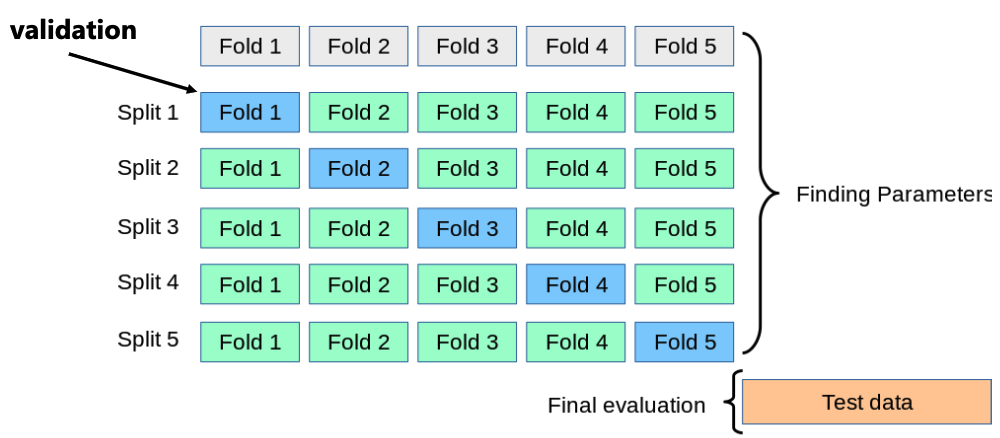
\includegraphics[width=0.83\linewidth]{Materials/crossValidation}
	\caption{Illustration of cross validation. Each of the blue splits are used at turn as validation sets, whereas the green splits are used training sets. Illustration taken from slides.}
	\label{crossVal}
\end{figure}
\section{Skin lesion classifier}
For the skin lesion competition I developed a model in collaboration with Marcus Hansen, Sarah Hansen and Ulrik Larsen. This model consists of six blocks of 3 by 3 convolutions with a ReLU activation function followed by a batch normalization followed by a 2 by 2 max pooling. For the convolutions padding with zeros have been used to keep the result after convolutions the same as the input size. After these six blocks, three blocks of a fully connected layer with a ReLU activation function followed by a batch normalization is used. The first fully connected layer has size 32, the second 16 and the last has 8. Lastly we have a fully connected layer of size 1 with a sigmoid activation function to get the class probability. This model has been trained with binary cross entropy as the loss function and an Adam optimizer with initial learning rate 0.00001. For the competition this model was trained for 1000 epochs using random affine transformations on the training data. The \textbf{final training accuracy} was around \textbf{0.90}, the \textbf{final validation accuracy} was around \textbf{0.80} and the \textbf{final test accuracy} was around \textbf{0.70}.\\
To evaluate this classification model I have been retraining the model, however, due to limitations in hardware I have only been able to train for 100 epochs. To compensate for this, I have used a learning rate of 0.0001 (a factor 10 larger) instead. The metrics I have chosen to use to evaluate the model are \textit{accuracy}, \textit{area under the ROC curve} and \textit{area under the precision / recall curve}. Accuracy simply tells us how many correctly classified images we got, i.e. true positives plus true negatives. Area under the ROC curve is given by measuring the area under the curve of a ROC curve. A ROC curve is made by plotting the sensitivity vs 1-specificity and tells us about the trade-off between the true positive rate and the false positive rate, i.e. the percentage of true positives we expect to find if we allow for some false positives. The area under the precision / recall curve is given by measuring the area under a precision / recall curve. Precision / recall curves measures how good the model is at predicting the positive class vs the ratio of true positives and false positives. Precision / recall curves can be relevant when we have imbalanced data, as the curve describes how often we predict true positive without introducing false negative, that is, we disregard the true negative 'accuracy'.

\begin{figure}
	\centering
	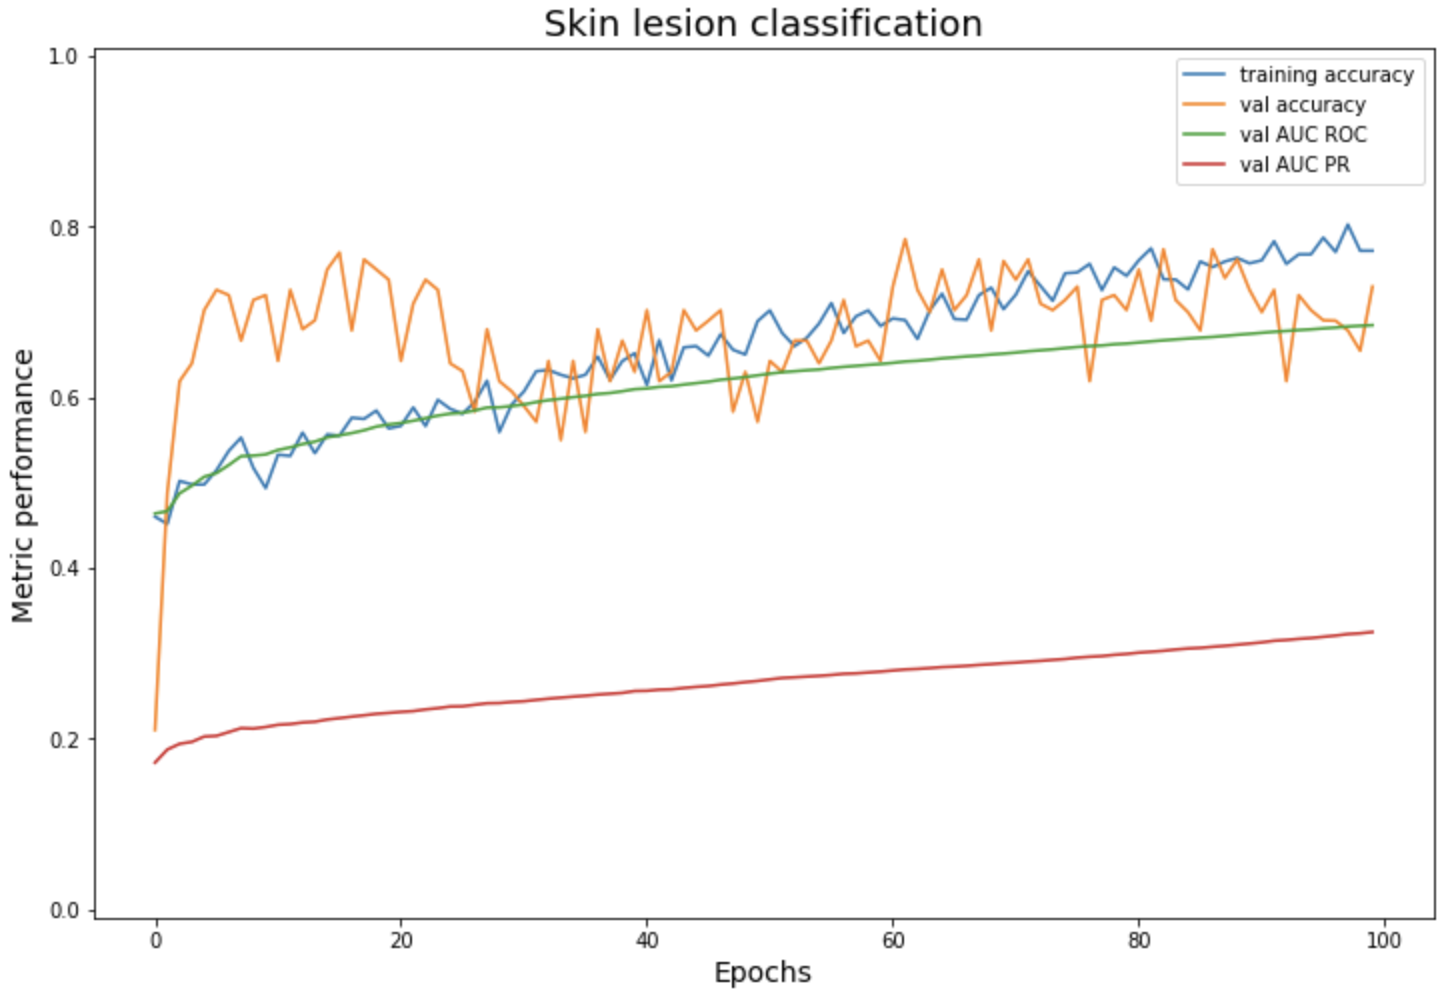
\includegraphics[width=0.88\linewidth]{Materials/skinlesion}
	\caption{Performance of the retrained skin lesion classifier.}
	\label{skinlesion}
\end{figure}
In \autoref{skinlesion} we see the training and validation accuracy along the area under the ROC curve and area under the precision / recall curve. We note these results are not as good as the results of the original model based on the validation accuracy. However, an accuracy of about 0.7 on unknown data is not ideal, but the model has learnt something. We note both the validation and training accuracy are still increasing and so, more epochs would probably have improved the model. When looking at area under the curve for ROC, we note it is steadily improving, which means we are getting better and better at predicting true positives without having to include more false positives. Lastly we note the area under the curve for precision / recall is also steadily increasing, which means we are getting better at predicting true positives without predicting false negatives. 
\section{Conclusion}
In conclusion we have seen where segmentation can be used in medical image analysis, we have seen the risks of dilation and erosion and explained the benefits of them, we have concluded Graph cut segmentations are preferred, but also have limited applications and Random walker alleviates these constrains by being non-deterministic, and finally we have looked into how PCA can be used for segmentation.
\newpage
%
% ---- Bibliography ----
%
% BibTeX users should specify bibliography style 'splncs04'.
% References will then be sorted and formatted in the correct style.
%
% \bibliographystyle{splncs04}
% \bibliography{mybibliography}
%
%\begin{thebibliography}{8}
%\bibitem{MIA}
%A.P. Dhawan, Medical Image Analysis, 2nd edition, 2011, John Wiley
%
%\bibitem{MIS}
%A. Maier, et al., Medical Imaging Systems, 2018, Springer Open
%
%\end{thebibliography}
\section{Code collaboration}
The code for this assignment has been developed in collaboration with Marcus Hansen, Sarah Hansen and Ulrik Larsen.
\end{document}
